\section{Regulador experto}
\label{sec:reg_expt}

Durante las producciones realizadas anteriormente, se ha notado que existe una relación entre la velocidad de tracción y el diámetro final del filamento, sin embargo, el sistema que se dispone carece de la robustez necesaria para poder trabajar con un regulador del tipo PID, en el que es necesario conocer de manera lo más exacta posible, la distribución de la planta con la que se trabaja.\\

Como se puede ver en la Figura \ref{fig:reg_mezcla}, la salida de filamento que proporciona el filastruder no es constante y en ocasiones, no está bien mezclada:

\begin{figure}[H]
    \centering
    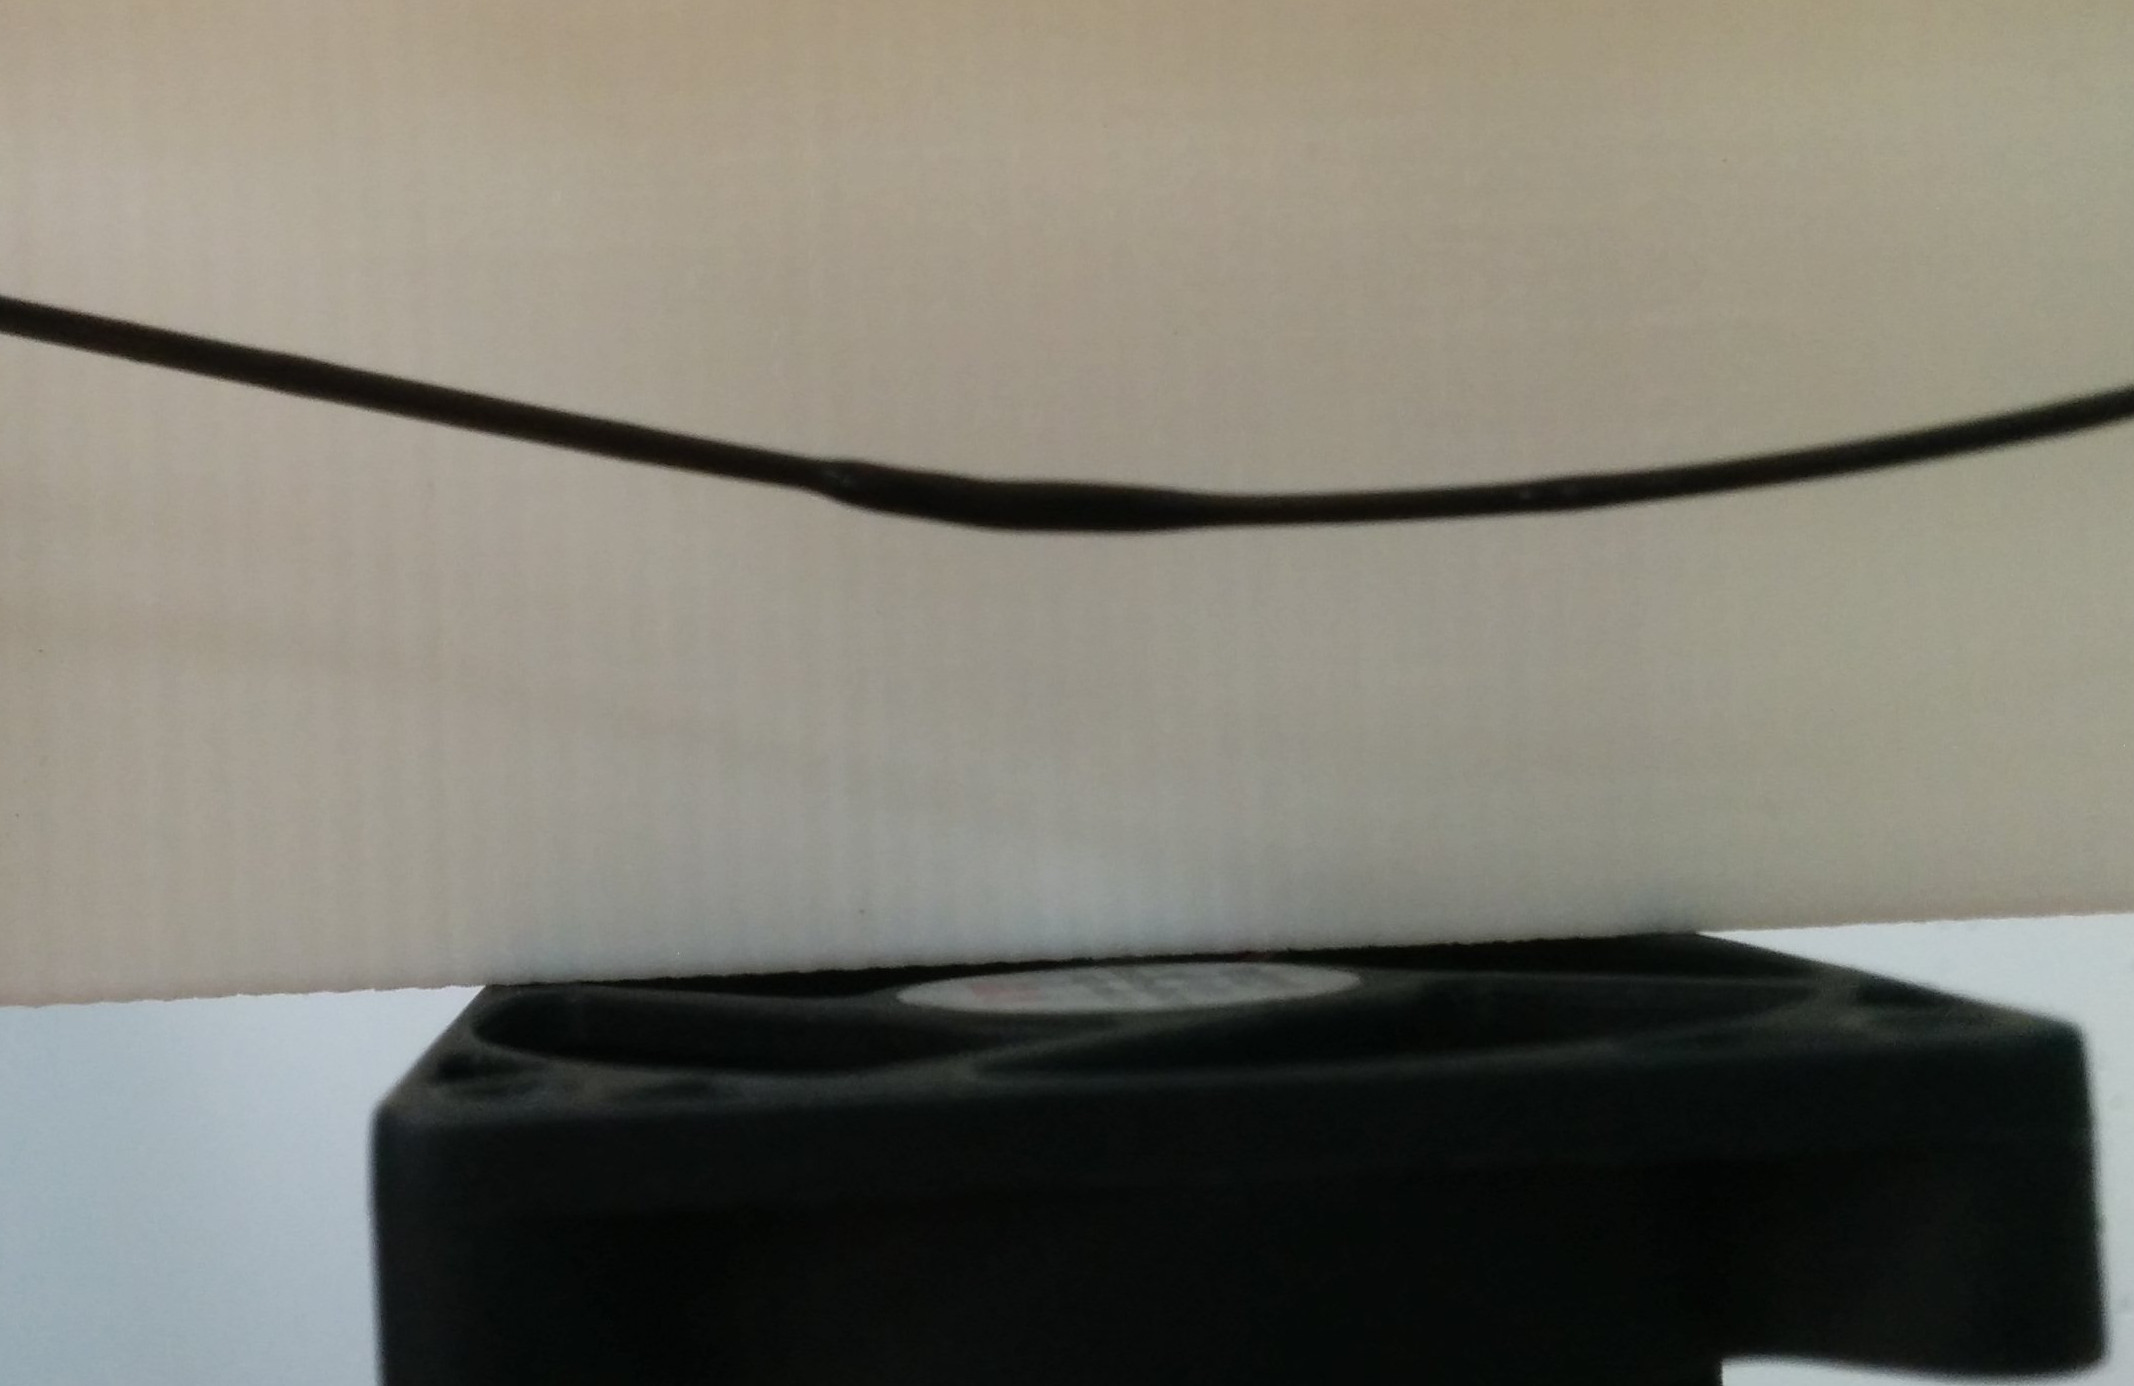
\includegraphics[width=0.6\textwidth]{images/producciones/22072015/IMG_20150722_120959.jpg}
    \caption[Mezcla incorrecta de la filastruder.]{Mezcla incorrecta de la filastruder. Algunos trozos de granza no son mezclados de forma correcta antes de salir del extrusor.}
    \label{fig:reg_mezcla}
\end{figure}

Por ello, se decide no usar un regulador PID e intentar implementar un regulador experto, el cual, imitará las acciones que un humano tomaría para resolver el problema. Este tipo de reguladores se basan en un conocimiento previamente adquirido por una persona, que ha trabajado con el sistema.\\

Para implementear este sistema, se definen una serie de reglas, en las que acotaremos los diámetros del filamento en regiones, y dependiendo, de si el diámetro crece o decrece, se actuará sobre la velocidad de tracción:

\begin{figure}[H]
    \centering
    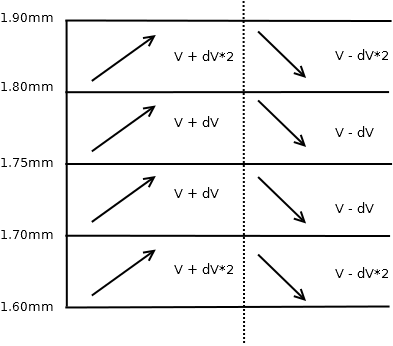
\includegraphics[width=0.5\textwidth]{images/producciones/11082015/Diagram1.png}
    \caption[Reglas a utilizar en el sistema experto.]{Reglas a utilizar en el sistema experto. En función de la zona en la que estemos aplicaremos un incremento positivo o negativo a la velocidad.}
    \label{fig:reg_reglas}
\end{figure}

En el anexo \ref{ane:resultados_regu} se detallan los ensayos realizados para comprobar la influencia del regulador en el diámetro.\\

Tomando como los datos obtenidos en el ensayo 4, como unos válidos para producción, vamos a pasar a compararlos con los datos obtenidos de dos fabricantes distintos de filamento, para ver posibles similitudes entre ellos.

\begin{table}[H]
	\centering
	\begin{tabular}{ccccccc}
		                    & BQ & FormFutura & Filastruder \\ \hline
		Medidas             & 291     &291    & 291      \\
		Media (mm)          & 1.75     & 1.70     & 1.74      \\
		Desviación estandar & 0.01     & 0.05     & 0.21      \\
		min(mm)             & 1.67     & 1.64     & 1.01      \\
		max(mm)             & 1.77     & 1.71     & 2.14     
	\end{tabular}
	\caption{Tabla comparativa de los resultados obtenidos}
	\label{tab:compara_results}
\end{table}

\begin{figure}[H]
    \centering
    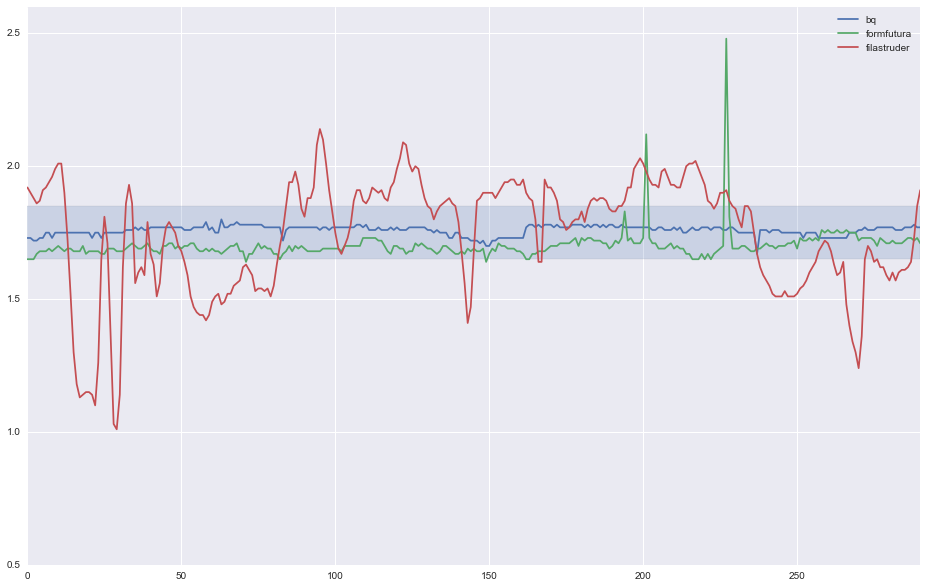
\includegraphics[width=0.99\textwidth]{images/producciones/conclusiones/output_8_1.png}
    \caption{Comparativa filamentos distintos fabricantes}
    \label{fig:concl_graf5}
\end{figure}

\begin{figure}[H]
    \centering
    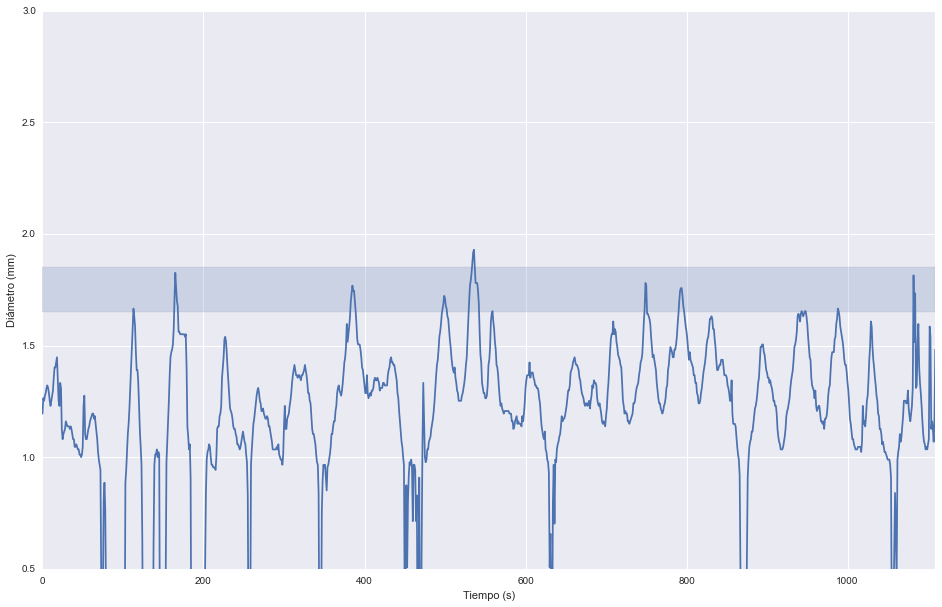
\includegraphics[width=0.6\textwidth]{images/producciones/conclusiones/output_9_1.png}
    \caption{Diagrama de cajas con diámetros de distintos fabricantes}
    \label{fig:concl_cajas5}
\end{figure}

Como podemos observar en los datos, el diámetro de los filamentos que proporcionan empresas como bq y formfutura, tienen unos valores mucho más estables que los nuestros. Lo cual es normal debido a la maquinaría y condiciones de trabajo que se han realizado en los experimentos.\\